% !Mode:: "TeX:UTF-8"
% !TEX program = xelatex
%%
%% Copyright 2007, 2008, 2009 Elsevier Ltd
%%
%% This file is part of the 'Elsarticle Bundle'.
%% ---------------------------------------------
%%
%% It may be distributed under the conditions of the LaTeX Project Public
%% License, either version 1.2 of this license or (at your option) any
%% later version.  The latest version of this license is in
%%    http://www.latex-project.org/lppl.txt
%% and version 1.2 or later is part of all distributions of LaTeX
%% version 1999/12/01 or later.
%%
%% The list of all files belonging to the 'Elsarticle Bundle' is
%% given in the file `manifest.txt'.
%%

%% Template article for Elsevier's document class `elsarticle'
%% with numbered style bibliographic references
%% SP 2008/03/01
%%
%%
%%
%% $Id: elsarticle-template-num.tex 4 2009-10-24 08:22:58Z rishi $
%%
%%
\documentclass[preprint,12pt,x11names,3p]{../templates/Elsevier/elsarticle}
\graphicspath{{figures/}}

%% Use the option review to obtain double line spacing
%% \documentclass[preprint,review,12pt]{elsarticle}

%% Use the options 1p,twocolumn; 3p; 3p,twocolumn; 5p; or 5p,twocolumn
%% for a journal layout:
%% \documentclass[final,1p,times]{elsarticle}
%% \documentclass[final,1p,times,twocolumn]{elsarticle}
%% \documentclass[final,3p,times]{elsarticle}
%% \documentclass[final,3p,times,twocolumn]{elsarticle}
%% \documentclass[final,5p,times]{elsarticle}
%% \documentclass[final,5p,times,twocolumn]{elsarticle}

%% if you use PostScript figures in your article
%% use the graphics package for simple commands
%% \usepackage{graphics}
%% or use the graphicx package for more complicated commands
%% \usepackage{graphicx}
%% or use the epsfig package if you prefer to use the old commands
%% \usepackage{epsfig}

%% The amssymb package provides various useful mathematical symbols
\usepackage{amssymb}
%% The amsthm package provides extended theorem environments
%% \usepackage{amsthm}

%% The lineno packages adds line numbers. Start line numbering with
%% \begin{linenumbers}, end it with \end{linenumbers}. Or switch it on
%% for the whole article with \linenumbers after \end{frontmatter}.
%% \usepackage{lineno}

%% natbib.sty is loaded by default. However, natbib options can be
%% provided with \biboptions{...} command. Following options are
%% valid:

%%   round  -  round parentheses are used (default)
%%   square -  square brackets are used   [option]
%%   curly  -  curly braces are used      {option}
%%   angle  -  angle brackets are used    <option>
%%   semicolon  -  multiple citations separated by semi-colon
%%   colon  - same as semicolon, an earlier confusion
%%   comma  -  separated by comma
%%   numbers-  selects numerical citations
%%   super  -  numerical citations as superscripts
%%   sort   -  sorts multiple citations according to order in ref. list
%%   sort&compress   -  like sort, but also compresses numerical citations
%%   compress - compresses without sorting
%%
%% \biboptions{comma,round}

% \biboptions{}


% \journal{Nuclear Physics B}

\begin{document}

\begin{frontmatter}

% !TEX root = Eco-Model.tex

\title{The Evolution of Manufacturing Ecosystem in Cloud Manufacturing Architecture
%Cloud Manufacturing Ecosystem - Scheduling And Evolving
}

\author[add1]{Shengkai Chen}
\author[add1,add2]{Shuiliang Fang\corref{cor1}}
% \ead{me_fangsl@zju.edu.cn}
% \address[label1]{ZJU}
% \address[label1]{Address One}
\address[add2]{The State Key Laboratory of Fluid Power Transmission and Control, College of Mechanical Engineering, Zhejiang University, Hangzhou, 310027, China}
\address[add1]{Key Laboratory of Advanced Manufacturing Technology of Zhejiang Province, College of Mechanical Engineering, Zhejiang University, Hangzhou , 310027, China}
% \author[a,b,*]{Third Author}

% \address[a]{First affiliation, Address, City and Postcode, Country}
% \address[b]{Second affiliation, Address, City and Postcode, Country}
% \fntext[label4]{Small city}

\cortext[cor1]{Corresponding author. Tel.: +86-135-8880-3980; Email: me\_fangsl@zju.edu.cn}

\begin{abstract}
In cloud manufacturing, individuals engage in manufacturing business through the well-designed platform, where provider provide manufacturing resource for demander to search and purchase it. This business model allows platform operator to manage distributed massive manufacturing resources, which may help provider reduce the idle rate of their resources.
However, in such manufacturing ecosystem, the heterogeneity attribute of resource makes it tough to classify them, and the chaotic operation mode makes it hard to meet demander's need.
Cloud manufacturing ecosystem has more complicated relationship among individuals in it than that in normal manufacturing system, one individual can make decisions depend on the surroundings and others' with the help of integrated advanced technologies. Thus, in this paper, we designed an original operation mode with 3 extensions for the cloud manufacturing ecosystem to help describe some decision makings in individuals and the platform operator.
With the help of Repast Simphony, we designed an agent-based simulation model and an experiment to validate the effectiveness of these operation modes. The experiment result shows: with incubation mode, the job queue length is reduced and the resource idle rate is declined; with outsourcing mode, the job queue length is also reduced but not as much as that with incubation mode and more resource is required; with metabolism mode, lower resource is required than that with other modes and resource idle rate just rose up a little. The combination of incubation and metabolism mode is one ideal mode to maintain the manufacturing ecosystem with.
\end{abstract}

\begin{keyword}
Cloud manufacturing ecosystem \sep
Resource servitization and optimization\sep
Operation mode\sep
Manufacturing evolution\sep
Agent-based simulation

\end{keyword}
% \belowfrontmatterskip0pt

\end{frontmatter}

%%
%% Start line numbering here if you want
%%
% \linenumbers

%% main text
% !TEX root = ../beamer.tex
\section{Introduction and Preliminary}

\subsection{Our Projects}

\begin{frame}{Introduction}{Our Projects}
  \begin{itemize}
  \item {
    My first point.
  }
  \item {
    My second point.
  }
  \end{itemize}
\end{frame}


\subsection{Operating Mode}

% You can reveal the parts of a slide one at a time
% with the \pause command:
\begin{frame}{Preliminary}{Operating Mode}
  \begin{itemize}
  \item {
    First item.
    \pause % The slide will pause after showing the first item
  }
  \item {   
    Second item.
  }
  % You can also specify when the content should appear
  % by using <n->:
  \item<3-> {
    Third item.
  }
  \item<4-> {
    Fourth item.
  }
  % or you can use the \uncover command to reveal general
  % content (not just \items):
  \item<5-> {
    Fifth item. \uncover<6->{Extra text in the fifth item.}
  }
  \end{itemize}
\end{frame}


% !TEX root = Eco-Model.tex
\section{Preliminaries} % (fold)
 
\subsection{Services and Tasks}
Resources and Services, Orders and Tasks,
Similary to the relation of service and resource, order and task 

transaction

\subsection{Roles}
Most recent studies like Wu et al.\cite{Wu2013} described the roles in Cloud Manufacturing as a tri-group model with:\begin{inparaenum}[1)]
\item Users/Customers,
\item Application providers and
\item Physical resource providers.
\end{inparaenum}
However, the roles in real world always not go like this model, since it parted roles only by their functions. While, users could get different function roles depend on what transaction they take, we should make some modifiacations on this model.

Before the emendation of the roles, some related standard name should be taken:
\begin{asparadesc}
\item[User] The main role in Cloud Manufacturing, which is combined of Seller and Buyer as shown in \autoref{tab:categoryuser}, usually acts as Seller or Buyer according to the specific transaction;
\item[Seller] The temporary role in a transaction, which provides the allocated part of manufacturing service and makes a evalution about the Buyer after the transaction;
\item[Buyer] The temporary role in a transaction, which submits the allocated part of manufacturing task and makes a evalution about the Seller after the transaction;
\item[Administrator] The role that gets the work for the operation and maintenance of the platform, has indirectly impact on the Ecosystem.
\end{asparadesc}
\begin{table}[htbp]
  \centering\small
  \caption{Category of Users}
    \begin{tabularx}{\textwidth}{llccX}
    \toprule
        &  & Seller & Buyer & Description \\
    \midrule
    Generalized & User & $\surd$ & $\surd$ & Act as Seller or Buyer according to the specific transaction. \\
    Enterprise & User & $\surd$ & &  Provides the allocated part of manufacturing services and makes a evalution about the Buyer after the transaction. \\
    Customer & User& & $\surd$ &  Submits the allocated part of manufacturing tasks and makes a evalution about the Seller after the transaction.\\
    \bottomrule
    \end{tabularx}%
  \label{tab:categoryuser}%
\end{table}%
As defined above, Enterprise User is the special case of the User(short for Generalized User) that purely provides manufacturing services and the Customer User is similarly defined.

Hence, there is only two roles in the Ecosystem worth to be studied: User and Administrator, the proportion of user type could be adjusted as the runtime of the system goes by.

\subsection{Operation Mode of Ecosystem}
The style the Cloud Manufacturing Ecosystem appears mainly depends on the way the operation mode takes, therefore, research on features and issues in the Ecosystem would be taken within the scope of operation mode we are going to set up. As shown in \autoref{fig:platformstruct}, the principal struct of Ecosystem can be described into four main branch, how these branches grow determines how the Operation Mode will come out, and it will be easy to figure out the specified mode we make with some flow charts.

\begin{figure}[!h]
\centering
\resizebox{0.7\textwidth}{!}{% !TEX root = ..\Eco-Model.tex
\begin{tikzpicture}
[mindmap,
every node/.style={concept, text=white, execute at begin node=\hskip0pt,circular drop shadow},
root concept/.append style={concept color=black, fill=white, line width=1ex, text=black, font=\Large\scshape},
grow cyclic,
level 1/.append style={level distance=4.5cm,sibling angle=90, font=\scshape},
level 2/.append style={level distance=3cm,sibling angle=45, font=\scriptsize\bf},
level 3/.append style={level distance=2cm,sibling angle=60, font=\scriptsize\bf},
level 4/.append style={level distance=1cm,sibling angle=60, font=\tiny\bf}]
\node [root concept] {Cloud Manufacturing Ecosystem}  % root
child [concept color = gray]{ node {Schedule}
child { node {Service Standardization}}
child { node {Decision Making Support}}
child { node {Platform Assistance}}
child { node {Match Regualtion}}
}
child [concept color = gray]{ node {User}
  child { node {Submit Order}}
  child { node {Provide Resource}}
  child { node {Make Transaction}}
  child { node {Evalute Others}}
  }
child [concept color = gray]{ node {Envolve}
  child { node {Optimization}
    child { node {Manufacturing}}
    child { node {Industrial Chain}}
    }
  child { node {Member}
    child { node {Introduce}}
    child { node {Eliminate}}
    }
  child { node {Adjust User Proportion}
    child { node {Rating}}
    child { node {Recommand}}
    }
  child { node {Development Guidance}}
  }
child [concept color = gray]{ node {Platform}
  child { node {Authority Control}}
  child { node {Transaction Bridge}}
  child { node {Dashbord}
    child { node {Service}}
    child { node {Task}}
    child { node {User}}
    }
child { node {Administrate}}
  child { node {Hub}
    child { node {Service}}
    child { node {Resource}}
    child { node {Ranking}}
    }
  child { node {Scheduling Assistance}}
}
;
\end{tikzpicture}}
\caption{Principal Struct of Cloud Manufacturing Ecosystem}
\label{fig:platformstruct}
\end{figure}

Because the metioned system is too complex to analyse in every detail, we focus on two important operation flows -- Order Flow and User Rank -- to help illustrate the Operation Mode. 

\subsubsection{Order Flow}
Each manufacturing order (order for short) appears when Users make transaction in the platform, it might then go through some different modules and a simple version of its flow was shown on \autoref{fig:orderflow}.

If an order accomplished smoothly, it will be constructed into tasks pieces in order to match the appropriate manufacturing services usually, similar to a large dataset processed with MapReduce\cite{Dean2008} schema. Then each piece could be processed by distributed resources with the outsourcing strategy User makes.

\begin{figure}[!h]
\centering\small
\subfloat[Order Flow]{\resizebox{0.45\textwidth}{!}{% !TEX root = flow_head.tex
\begin{tikzpicture}[%
    >=triangle 60,              % Nice arrows; your taste may be different
    start chain=going below,    % General flow is top-to-bottom
    node distance=6mm and 60mm, % Global setup of box spacing
    every join/.style={norm},   % Default linetype for connecting boxes
    ]
% ------------------------------------------------- 
% A few box styles 
% <on chain> *and* <on grid> reduce the need for manual relative
% positioning of nodes
\tikzset{
  base/.style={draw, on chain, on grid, align=center, minimum height=4ex},
  proc/.style={base, rectangle, text width=8em},
  test/.style={base, diamond, aspect=2, text width=5em},
  term/.style={proc, rounded corners},
  % coord node style is used for placing corners of connecting lines
  coord/.style={coordinate, on chain, on grid, node distance=6mm and 25mm},
  % nmark node style is used for coordinate debugging marks
  nmark/.style={draw, cyan, circle, font={\sffamily\bfseries}},
  % -------------------------------------------------
  % Connector line styles for different parts of the diagram
  norm/.style={->, draw, lcnorm},
  free/.style={->, draw, lcfree},
  cong/.style={->, draw, lccong},
  it/.style={font={\small\itshape}}
}
% -------------------------------------------------
% Start by placing the nodes
\node [term] {Be Submitted};
\end{tikzpicture}}\label{fig:orderflow}} \hspace{0.09\textwidth}
\subfloat[User Rank]{\resizebox{0.45\textwidth}{!}{% !TEX root = flow_head.tex
\begin{tikzpicture}[%
    >=triangle 60,              % Nice arrows; your taste may be different
    start chain=going below,    % General flow is top-to-bottom
    node distance=6mm and 60mm, % Global setup of box spacing
    every join/.style={norm},   % Default linetype for connecting boxes
    ]
% ------------------------------------------------- 
% A few box styles 
% <on chain> *and* <on grid> reduce the need for manual relative
% positioning of nodes
\tikzset{
  base/.style={draw, on chain, on grid, align=center, minimum height=4ex},
  proc/.style={base, rectangle, text width=8em},
  test/.style={base, diamond, aspect=2, text width=5em},
  term/.style={proc, rounded corners},
  % coord node style is used for placing corners of connecting lines
  coord/.style={coordinate, on chain, on grid, node distance=6mm and 25mm},
  % nmark node style is used for coordinate debugging marks
  nmark/.style={draw, cyan, circle, font={\sffamily\bfseries}},
  % -------------------------------------------------
  % Connector line styles for different parts of the diagram
  norm/.style={->, draw, lcnorm},
  free/.style={->, draw, lcfree},
  cong/.style={->, draw, lccong},
  it/.style={font={\small\itshape}}
}
% -------------------------------------------------
% Start by placing the nodes
\node [term]              (m1)  {Be Introduced};
\node [proc, join]        (p8)  {Get Initial Rank $R$};
\node [coord, yshift=2mm] (c1)  {}; \cmark{1}
\node [test, yshift=2mm]  (t1)  {Transact?};
\node [proc, yshift=-3mm] (p1)  {Increase $R$};


\node [proc, right=of t1] (p4)  {Wait};
\node [proc]              (p5)  {Compete to Get Task};
\node [test, join]        (t5)  {Make it?};
\node [coord, yshift=2mm] (c3)  {}; \cmark{3}

\node [test, yshift=2mm]  (t6)  {Outsourcing?};
\node [test]              (t7)  {Partly or Whole?};
\node [proc]              (p6)  {Submit Outsourcing Request};
\node [proc]              (p7)  {Decrease $R$};
\node [test, join]        (t8)  {$R < R_{base}$?};
\node [term]              (m2)  {Eliminate};

\node [test, left=of c3]  (t2)  {All Tasks Accomplished?};
\node [proc]              (p2)  {Process Task};
\node [test]              (t3)  {Accepted?};
\node [proc]              (p3)  {Pass the Outsouring Task};
\node [test]              (t4)  {Task Accomplished?};

\node [coord, left=of p1](c2)  {}; \cmark{2}

\draw [->, lcnorm] (p4) |- (c1);
\draw [->, lcnorm] (p8) -- (t1);
\draw [->, lcnorm] (p1) --(c2) |- (c1);

\path (t1.east)   to node [near start, yshift=1em] {$n$} (p4);
\path (t1.south) to node [near start, xshift=1em] {$y$} (p1);
  \draw [o->, lcnorm] (t1.east) -- (p4);
  \draw [*->, lcnorm] (t1.south) |- (p5);

\end{tikzpicture}}\label{fig:userrank}}
\caption{ Primary Flow Chart of Order and User}
\end{figure}
\subsubsection{User Rank}
Apart from the above mentioned order related behavior, User can also submit resources, change standrd, make recommandation and so on, according to the permission degree the User has. User Rank provides the basis to set the permission degree, it gets the initial value when User was introduced in the system and it will increase or decrease by good or bad performance in each transaction, the follow equation shows a simple way to evaluate the User Rank. 

\begin{equation}
  \begin{cases}
      Rank_{[T+1]} = Rank_{[T]} + Gain - Lose, & T \geqslant 1\\
      Rank_{[0]} = Rank_{[init]}
  \end{cases}
\label{equ:simplerank}
\end{equation}
Subscript $T$ in \eqref{equ:simplerank} counts the transaction User takes. \autoref{sub:rating_schema}

User Rank will be adjusted all the time only if the User was eliminated for a low rank value, the adjustment was based on the evalution messages, which seller and buyer would post after each transaction, basically. Introduction and elimination of User implies the evolution of the Cloud Manufacturing Ecosystem. 

\subsubsection{Platform}
Need a picture with cms run pic

provide the method of order - > task , resources -> service
gain the evalution messages for analysis
decide to introduce or eliminate.

\subsection{Data Science Tools}


simply descript some related tools and where to use.

% !TEX root = Eco-Model.tex
\section{Methodological approach} % (fold)
\label{sec:methodological_approach}

This section starts with a brief overview of ABMS. Then .... Finally ... 
i.e. the swarm model of the system.

In a word, the center of the research is the design of the user agent, and the core of the agent is to make decisions. so the core of the evolution is to make decision? 

core of the paper: agent simulation, decision making.

\subsection{Framework of Agent-based modeling} % (fold)
\label{sub:framework of agent based modeling}
\begin{figure}[htbp]
\centering\small
\subfloat[Order Flow]{\resizebox{0.45\textwidth}{!}{% !TEX root = flow_head.tex
\begin{tikzpicture}[%
    >=triangle 60,              % Nice arrows; your taste may be different
    start chain=going below,    % General flow is top-to-bottom
    node distance=6mm and 60mm, % Global setup of box spacing
    every join/.style={norm},   % Default linetype for connecting boxes
    ]
% ------------------------------------------------- 
% A few box styles 
% <on chain> *and* <on grid> reduce the need for manual relative
% positioning of nodes
\tikzset{
  base/.style={draw, on chain, on grid, align=center, minimum height=4ex},
  proc/.style={base, rectangle, text width=8em},
  test/.style={base, diamond, aspect=2, text width=5em},
  term/.style={proc, rounded corners},
  % coord node style is used for placing corners of connecting lines
  coord/.style={coordinate, on chain, on grid, node distance=6mm and 25mm},
  % nmark node style is used for coordinate debugging marks
  nmark/.style={draw, cyan, circle, font={\sffamily\bfseries}},
  % -------------------------------------------------
  % Connector line styles for different parts of the diagram
  norm/.style={->, draw, lcnorm},
  free/.style={->, draw, lcfree},
  cong/.style={->, draw, lccong},
  it/.style={font={\small\itshape}}
}
% -------------------------------------------------
% Start by placing the nodes
\node [term] {Be Submitted};
\end{tikzpicture}}\label{fig:orderflow}} \hspace{0.09\textwidth}
\subfloat[User Rank]{\resizebox{0.45\textwidth}{!}{% !TEX root = flow_head.tex
\begin{tikzpicture}[%
    >=triangle 60,              % Nice arrows; your taste may be different
    start chain=going below,    % General flow is top-to-bottom
    node distance=6mm and 60mm, % Global setup of box spacing
    every join/.style={norm},   % Default linetype for connecting boxes
    ]
% ------------------------------------------------- 
% A few box styles 
% <on chain> *and* <on grid> reduce the need for manual relative
% positioning of nodes
\tikzset{
  base/.style={draw, on chain, on grid, align=center, minimum height=4ex},
  proc/.style={base, rectangle, text width=8em},
  test/.style={base, diamond, aspect=2, text width=5em},
  term/.style={proc, rounded corners},
  % coord node style is used for placing corners of connecting lines
  coord/.style={coordinate, on chain, on grid, node distance=6mm and 25mm},
  % nmark node style is used for coordinate debugging marks
  nmark/.style={draw, cyan, circle, font={\sffamily\bfseries}},
  % -------------------------------------------------
  % Connector line styles for different parts of the diagram
  norm/.style={->, draw, lcnorm},
  free/.style={->, draw, lcfree},
  cong/.style={->, draw, lccong},
  it/.style={font={\small\itshape}}
}
% -------------------------------------------------
% Start by placing the nodes
\node [term]              (m1)  {Be Introduced};
\node [proc, join]        (p8)  {Get Initial Rank $R$};
\node [coord, yshift=2mm] (c1)  {}; \cmark{1}
\node [test, yshift=2mm]  (t1)  {Transact?};
\node [proc, yshift=-3mm] (p1)  {Increase $R$};


\node [proc, right=of t1] (p4)  {Wait};
\node [proc]              (p5)  {Compete to Get Task};
\node [test, join]        (t5)  {Make it?};
\node [coord, yshift=2mm] (c3)  {}; \cmark{3}

\node [test, yshift=2mm]  (t6)  {Outsourcing?};
\node [test]              (t7)  {Partly or Whole?};
\node [proc]              (p6)  {Submit Outsourcing Request};
\node [proc]              (p7)  {Decrease $R$};
\node [test, join]        (t8)  {$R < R_{base}$?};
\node [term]              (m2)  {Eliminate};

\node [test, left=of c3]  (t2)  {All Tasks Accomplished?};
\node [proc]              (p2)  {Process Task};
\node [test]              (t3)  {Accepted?};
\node [proc]              (p3)  {Pass the Outsouring Task};
\node [test]              (t4)  {Task Accomplished?};

\node [coord, left=of p1](c2)  {}; \cmark{2}

\draw [->, lcnorm] (p4) |- (c1);
\draw [->, lcnorm] (p8) -- (t1);
\draw [->, lcnorm] (p1) --(c2) |- (c1);

\path (t1.east)   to node [near start, yshift=1em] {$n$} (p4);
\path (t1.south) to node [near start, xshift=1em] {$y$} (p1);
  \draw [o->, lcnorm] (t1.east) -- (p4);
  \draw [*->, lcnorm] (t1.south) |- (p5);

\end{tikzpicture}}\label{fig:userrank}}
% \resizebox{0.9\textwidth}{!}{% !TEX root = ../Eco-Model.tex
\begin{tikzpicture}[%
    >=triangle 60,              % Nice arrows; your taste may be different
    start chain=going right,    % General flow is top-to-bottom
    node distance=6mm and 10mm, % Global setup of box spacing
    every join/.style={norm},   % Default linetype for connecting boxes
    ]
% ------------------------------------------------- 
% A few box styles 
% <on chain> *and* <on grid> reduce the need for manual relative
% positioning of nodes
\tikzset{
  base/.style={draw, on chain, on grid, align=center, rectangle},
  proc/.style={base, text width=6em, minimum height=8em},
  term/.style={base, text width=5em, rounded corners, minimum height = 3ex},
  dproc/.style={proc, minimum height = 20ex},
  gathe/.style={draw, on chain, on grid, align=center, circle, minimum height=4ex, text width=0.5em, node distance=10mm and 8mm},
  % coord node style is used for placing corners of connecting lines
  coord/.style={coordinate, on chain, on grid, node distance=6mm and 25mm},
  sky/.style={coordinate, on chain, on grid, node distance=6mm and 60mm},
  % nmark node style is used for coordinate debugging marks
  nmark/.style={draw, cyan, circle, font={\sffamily\bfseries}},
  % -------------------------------------------------
  % Connector line styles for different parts of the diagram
  norm/.style={->, draw, lcnorm},
  free/.style={->, draw, lcfree},
  cong/.style={->, draw, lccong},
  it/.style={font={\small\itshape}}
}
% -------------------------------------------------
% Start by placing the nodes
\node [term, fill = lcfree!25]              {Order};
\node [proc, join=by free]  (p1) {Task Hub};
\node [proc, dashed] (d) {};
\node [term, xshift = 12mm] (oc) {Order Check};
\node [term, join=by cong, fill = lccong!25]  {Submit};

\node [gathe, right=of d,yshift=5mm, xshift= 15mm] (g1) {};
\node [term, below=of d, yshift=15.5mm] (u1) {User 1};
\node [term, below=of u1] (u2) {User 2};
\node [below=-1mm of u2] (u3) {$\vdots$};
\node [term,below=of u3, yshift=-1mm] (u4) {User n};
\node [below=of u4,yshift=2.6mm] {User Cluster};
\node [gathe, below=of g1] (g2) {};
\node [coord, above=of g1, yshift=8mm] (c1) {};

\draw [->, lccong] (g2) -- (oc.west);
\draw [->, lcnorm] (p1) -- (u1.west);
\draw [->, lcnorm] (p1) -- (u2.west);
\draw [->, lcnorm] (p1) -- (u4.west);

\draw [->, lcnorm] (u1.east) -- (g1.west);
\draw [->, lccong] (u1.east) -- (g2.west);
\draw [->, lcnorm] (u2.east) -- (g1.west);
\draw [->, lccong] (u2.east) -- (g2.west);
\draw [->, lcnorm] (u4.east) -- (g1.west);
\draw [->, lccong] (u4.east) -- (g2.west);
\draw [->, lcnorm] (g1) -- (c1) -- node [black, near end, yshift=0.75em, it]
    {(Outsourcing)} ++(-3.5cm,0) -| (p1) ;

\end{tikzpicture}}
\caption{Simple Flow Chart of Order}
% \label{fig:simpleorderflow}
\end{figure}

\subsubsection{Assumptions and notation}
\begin{itemize}
    \item one provider can publish only one order at one time;
    \item service quality give the initial rank, the product quality depends on the service quality, review depends on the service quality, and the rank depends on the review;
    \item when it comes to rank value, we refer two different rank values: user rank(provider) and service rank, their relationship should be determined.
\end{itemize}


\subsection{Agents in the ecosystem model} % (fold)
\label{sub:agents_in_the_ecosystem_model}
Using UML 
% subsection agents_in_the_ecosystem_model (end)

\subsubsection{Meta agent} % (fold)
\label{ssub:meta_agent}
is a decision maker
% subsubsection meta_agent (end)

\subsubsection{Demander agent} % (fold)
\label{ssub:demander_agent}
After pricing, chose the provider and the amount considering the time limit of the project and the budget.
% subsubsection demander_agent (end)

\subsubsection{Provider agent} % (fold)
\label{ssub:provider_agent}
Pricing function specify two main parts:
unit cost and
provided amount
% subsubsection provider_agent (end)

\subsubsection{Complex user agent} % (fold)
\label{ssub:complex_user_agent}

% subsubsection complex_user_agent (end)

\subsubsection{Platform agent} % (fold)
\label{ssub:platform_agent}
matching the 
\begin{figure}

\begin{tikzpicture}
\begin{class}[text width=8cm]{Job}{0,0}
    \attribute{needCapacity : Map}
    \operation{lala(haha): void}
\end{class}
\end{tikzpicture}
\caption{Test UML Diagram}

\end{figure}
% subsubsection platform_agent (end)


\subsection{Ecosystem model} % (fold)
\label{sub:ecosystem model}

% subsection model_realization (end)

\subsubsection{Design philosophy} % (fold)
\label{ssub:design_philosophy}
platform create demander and provider
demander, a subclass of user, generate need i.e. create order (the defined task bunch)
    task is a subclass of job, need to be processed with specified resource type and amount(type,amount) , have its process time.
provider, a subclass of user, provider resource with different type and capacity, these resources can be allocated to task job and service-call job, service-call is subclass of job, which is the job to combined to create service.

the two type of job, task and service call, have something in common that need to be processd with resource. for task, the resource is renewable, for service-call, the resource is unrenewable.

service can be generated after the finish of service-call, so it belongs to the user who generate the service-call. service more like a contract

service-call come out driven by the task need, when a task appears frequently, provider proposed the job that have the same configuration. so the service generated by the service-call will suit for the specificed task.

good for service: efficieny, do not have to coordinated anymore, flexibe wile process with task, with the outsource trick, slice the taks, co-worked by all the useful resources.
bad for service: task-oriented, can only process specified task,

% subsubsection design_philosophy (end)

\subsubsection{Main functions} % (fold)
\label{ssub:main_functions}
service - task outsource
% subsubsection main_functions (end)

\subsubsection{Main problem} % (fold)
\label{ssub:main_problem}

% subsubsection main_problem (end)

\subsubsection{Main flow design} % (fold)
\label{ssub:main_flow_design}
\begin{itemize}
    \item generate provider and demander
    \item generate order (with task)
    \item generate resources
    \item process tasks (with only resource)
    \item organize service
    \item process task (plus service)
    \item Review and elimination of provider and service
\end{itemize}
% subsubsection main_flow_design (end)

\subsubsection{Main modules design}
\label{subsub:main_modules}
inherent relationships, execution sequence/queue.

for service provider to modify their service area, i.e. breadth and depth.

Decision making involves choosing some course of action among various alternatives. For a decision maker, fulfilling the con

\subsubsection{System Model}
\begin{itemize}
    \item Co-evolution
    \item Self-organization
    \item Emergence 
    \item Adaption
\end{itemize}

Assumptions:
\begin{enumerate}
    \item substitute transport with time consume
    \item manufacturing agent randomly show up in the map
\end{enumerate}

Co-evolution consist of:
\begin{itemize}
    \item Scarcity of customers
    \item Conscious choice that enables the organizations to change
    \item Interconnectedness of the enables the organizations to change
    \item Feedback processes that carry the long-term consequences of co-evolution
\end{itemize}

% subsection modeling (end)

\subsection{Simulation design} % (fold)
\label{sub:simulation_design}

% subsection simulation_design (end)

\subsection{Agent-based modeling and simulation} % (fold)
\label{sub:agent_based_modeling_and_simulation}
\subsubsection{Agent design}

\subsubsection{Logical process}

\subsubsection{Interaction among agents}
some mathematical formulation display here to describe the whole ecosystem wide phenomenon, like Little formulation.


% subsection agent_based_model_and_simulation (end)
% section methodological_approach (end)
% !TEX root = Eco-Model.tex
\section{Experiment and result Analysis} % (fold)
\label{sec:Experiment_results}

Entities in the manufacturing ecosystem we designed above have these traits: \begin{inparaenum}[1)]
\item autonomous and self-directed, 
\item social, interacting with other entities, 
\item controlled by the environment, 
\item self-contained.
\end{inparaenum} They optimize their multi-objective decision makings to interact with others and the environment, hence, agent-based modeling and simulation(ABMS) technique\cite{Macal2009,north2007managing} is suitable for the study of the complex system. With the help of Repast Simphony\cite{North2013} package, we realized the ecosystem model and performed some experiments on it.

% \subsection{Agent-based modeling and simulation design} % (fold)
% \label{sub:agent_based_modeling_and_simulation}
% \subsubsection{Model realization}
% \begin{asparaenum}
% \item Main agents
% \suspend{asparaenum}
% \begin{figure}[htbp]
% \centering
% \tiny
% \subfloat[Job related classes]{\begin{tikzpicture}
%     % !TEX root = flow_head.tex

\begin{class}[text width=8cm]{Job}{0,0}
	\attribute{+ allocated: boolean}
	\attribute{+ allocation: Map}
	\attribute{+ candidates: Map}
	\attribute{+ inNeed: boolean}
	\attribute{+ needResourceCapacity: Map}
	\attribute{+ predecessor: Set}
	\attribute{+ prepareStatus: Map}
	\attribute{- processBehavior: ProcessBehavior}
	\attribute{- selectBehavior: SelectBehavior}
	\operation{+ addCandidates(competitor: Machine): void}
	\operation{+ CheckStatus(): void}
	\operation{+ Need(): void}
	\operation{+ Review(m: Machine): void}
	\operation{+ Select(watchedAgent: Job): void}
\end{class}


%     % !TEX root = flow_head.tex

\begin{class}[text width=8cm]{Task}{0,0}
	\attribute{+ master: Order}
	\attribute{+ owner: Map}
	\attribute{+ pause: boolean}
	\attribute{+ processingTime: int}
	\attribute{+ remainingTime: int}
	\attribute{+ type: Strihng}
	\operation{+ Task()}
	\operation{+ addOwner(user: User, p: int): void}
	\operation{+ CheckStatus(): void}
	\operation{+ Process(watchedAgent: Task): void}
	\operation{+ setParameters(taskData: Map): void}
\end{class}
%     % !TEX root = flow_head.tex

\begin{class}[text width=.225\textwidth]{ServiceCall}{1.08,-3.7}
	\inherit{Job}
	\attribute{+ owner: Provider}
	\attribute{+ type: String}
	\operation{+ ServiceCall()}
	\operation{+ setParameter(scData: Map): void}
	\operation{+ Recall(): void}
\end{class}
%     \end{tikzpicture}
%     \label{fig:jobclassed}}\hspace{1pt}
% \subfloat[Machine related classes]{\begin{tikzpicture}
%     % !TEX root = flow_head.tex

\begin{class}[text width=.45\textwidth]{Machine}{0,0}
	\attribute{+ assignBehavior: AssignBehavior}
	\attribute{+ buffer: List}
	\attribute{+ competeList: List}
	\attribute{+ jobList: List}
	\attribute{+ owner: Provider}
	\attribute{+ releaseBehavior: ReleaseBehavior}
	\attribute{+ responseBehavior: ResponseBehavior}
	\attribute{+ responseList: List}
	\attribute{+ type: String}
	\operation{+ Assign(t: Task): void}
	\operation{+ Release(j: Job): void}
	\operation{+ Reply(watchedAgent: Job): void}
	\operation{+ Response(watchedAgent: Task): void}
	\operation{+ Review(j: Job):void}
\end{class}


%     % !TEX root = flow_head.tex

\begin{class}[text width=.45\textwidth]{Resource}{-2.4,-3.66}
	\inherit{Machine}
	\attribute{+ available: int}
	\attribute{+ capacity: int}
	\attribute{+ master: Map}
	\attribute{+ needCap: Map}
	\attribute{+ sourceable: int}
	\operation{+ Resource()}
	\operation{+ addMaster(ser: Service, amonut: int): void}
	\operation{+ Assign(sc: ServiceCall, amount: int): void}
	\operation{+ Response(watchedAgent: ServiceCall): void}
\end{class}
%     % !TEX root = flow_head.tex

\begin{class}[text width=.45\textwidth]{Service}{2.4,-3.66}
	\inherit{Machine}
	\attribute{+ resourceComposition: Map}
	\operation{+ Service()}
	\operation{+ OutSource(): void}
\end{class}
%     \end{tikzpicture}
%     \label{fig:machineclassed}}\\
% \subfloat[User related classes]{\begin{tikzpicture}
%     % !TEX root = flow_head.tex

\begin{class}[text width=.45\textwidth]{User}{0,0}
	\attribute{- agentIDCounter: long}
	\attribute{\# agentID: String}
\end{class}
%     % !TEX root = flow_head.tex

\begin{class}[text width=.45\textwidth]{Provider}{-2.4,-1.2}
	\inherit{User}
	\attribute{+ candidates: List}
	\attribute{+ rank: double}
	\attribute{+ resourceList: List}
	\attribute{+ serviceList: List}
	\operation{+ GenerateResource(): void}
	\operation{+ GenerateService(serviceData: List): void}
	\operation{+ GenerateServiceCall(): void}
	\operation{+ RemoveServiceCall(sc: ServiceCall): void}
	
\end{class}
% % !TEX root = flow_head.tex

\begin{class}[text width=.45\textwidth]{Demander}{2.4,-1.2}
	\inherit{User}
	\attribute{+ orderList: List}
	\attribute{+ taskMap: Map}
	\operation{+ GenerateOrder(orderID: String): void}
	\operation{+ ReadData(orderID: String): void}
\end{class}


%     \end{tikzpicture}\label{fig:userclassed}}\hspace{3pt}
% \subfloat[Cloud Platform]{\begin{tikzpicture}
% 	% !TEX root = flow_head.tex

\begin{class}[text width=8cm]{CloudPlatform}{0,0}
	\attribute{- agentIDCounter: long}
	\attribute{\# agentID: String}
	\attribute{+ finishCount: int}
	\attribute{+ userList: List}
	\operation{+ CreateProvider(): void}
	\operation{+ CreateDemander(): void}
\end{class}


% 	\end{tikzpicture}\label{fig:platform}}
% \end{figure}


% \resume{asparaenum}
% \item Behavior interfaces and classes
% \end{asparaenum}

% \begin{figure}[htbp]
%     \centering
%     \tiny
%     \begin{tikzpicture}
%     % !TEX root = flow_head.tex

\begin{interface}[text width=.45\textwidth]{AssignBehavior}{0,0}
	\operation{+ BufferEnterance(t: Task, m: Machine): boolean}
	\operation{+ Queue(j: Job, m: Machine): void}
	\operation{+ Buff(t: Task, m: Machine): void}
\end{interface}


%     % !TEX root = flow_head.tex

\begin{interface}[text width=.45\textwidth]{SelectBehavior}{0,-1.7}
	\operation{+ Allocate(theOnes: Map): Map}
	\operation{+ Assign(allocation: Map, j: Job): void}
	\operation{+ Evaluation(j: Job, candidates: List): void}
	\operation{+ Select(j: Job, candidates: List): void}
\end{interface}
%     % !TEX root = flow_head.tex

\begin{interface}[text width=.45\textwidth]{ResponseBehavior}{0,0}
	\operation{+ Exist(j: Job, m: Machine): boolean}
\end{interface}
%     % !TEX root = flow_head.tex

\begin{interface}[text width=.45\textwidth]{ProcessBehavior}{4.8,-2.35}
	\operation{+ Process(j: Job): void}
\end{interface}
%     % !TEX root = flow_head.tex

\begin{interface}[text width=8cm]{ReleaseBehavior}{0,0}
	\operation{+ Release(j: Job, m: Machine): void}
	\operation{+ Next(m: Machine): void}
\end{interface}
%     % % !TEX root = flow_head.tex

\begin{class}[text width=8cm]{ServiceAssign}{0,0}
	\operation{+ BufferEnterance(t: Task, m: Machine): boolean}
	\operation{+ Queue(j: Job, m: Machine): void}
	\operation{+ Buff(t: Task, m: Machine): void}
\end{class}
%     % % !TEX root = flow_head.tex

\begin{class}[text width=.45\textwidth]{ResourceAssign}{2.4,-2.5}
	\implement{AssignBehavior}
	\operation{+ Buff(t: Task, m: Machine): void}
	\operation{+ BufferEnterance(t: Task, m: Machine): boolean}
	\operation{+ Queue(j: Job, m: Machine): void}
\end{class}
%     \end{tikzpicture}
%     \caption{Assign interface and related classes}
%     \label{fig:assigninterface}
% \end{figure}


\subsection{Experiments} % (fold)
\label{ssub:case_design}
We use the RanGen\cite{Demeulemeester2003} to generate order dataset in the well-known Patterson format with the parameters setting listed in \autoref{tab:generalparameter}. 
\begin{table}[htbp]
  \centering
  \scriptsize
  \caption{Order generating parameters setting}
    \begin{tabular}{cccccccccc}
    \toprule
    \textbf{$n_a$} & \textbf{OS} & \textbf{CI} & \textbf{$n_r$} & \textbf{RF} & \textbf{RC} & \textbf{$\lambda_d$} &\textbf{$\lambda_p$} & \textbf{$C_{k,0}$}\\
    \midrule
     10  &   0.3    &  [2,3]     &   12     &  0.3     &   0.5  & 0.2 & 0.3  & [20,30] \\
    \bottomrule
    \end{tabular}%
    {\footnotetext{\tiny The meaning of the first 5 parameters are defined in \cite{Demeulemeester2003}, $\lambda$ is the parameters of the arrival of user in simulation, $C_{k,0}$ is the initial capacity for $mr_k$}
    }
  \label{tab:generalparameter}%
\end{table}%
We assume provider and demander are arriving as the poisson process, in order to make sure the coming need resource capacity rate will not exceed the coming resource capacity rate in average to prevent the task explosion, we make sure that:
\begin{equation}
\lambda_d n_a n_r \cdot RF \cdot RC < \lambda_p \bar C_{k,0} \label{eq:balance}
\end{equation}

We design experiments to validate incubation, outsourcing and metabolism mode \autoref{tab:grouping}, 10 datasets represent 10 types of orders, each of them contains 10 tasks with different configuration on 12 types of resources to perform with. 

\begin{table}[htbp]
  \centering
  \scriptsize
  \caption{Experiments mode grouping}
    \begin{tabular}{llcc}
    \toprule
          &       & Without metabolism & With metabolism \\
    \midrule
    \multicolumn{2}{l}{Resource-only} & Mode 11 & Mode 12 \\\hline
    \multicolumn{1}{l}{\multirow{2}[0]{*}{Service-incubate}} & without outsource & Mode 21 &Mode 22 \\\cline{2-4}
    \multicolumn{1}{l}{} & with outsource & Mode 31 & Mode 32 \\
    \bottomrule
    \end{tabular}%
  \label{tab:grouping}%
\end{table}%
% subsubsection parameters_setting (end)

\subsection{Result and analysis} % (fold)
\label{ssub:result_and_analysis}
All the experiments are simulated with same random seed to make no difference on the coming of order, provider and other irrelevant configuration to our validation.  After bunch of experiments with different random seeds, we discovered some laws in operation mode. Take random seed 776189616 as example, we run the simulation for 6000 tick time and the experiment's results are displayed in \autoref{fig:out} and \autoref{tab:averagevalue},
\begin{figure}[htbp]
    \centering
    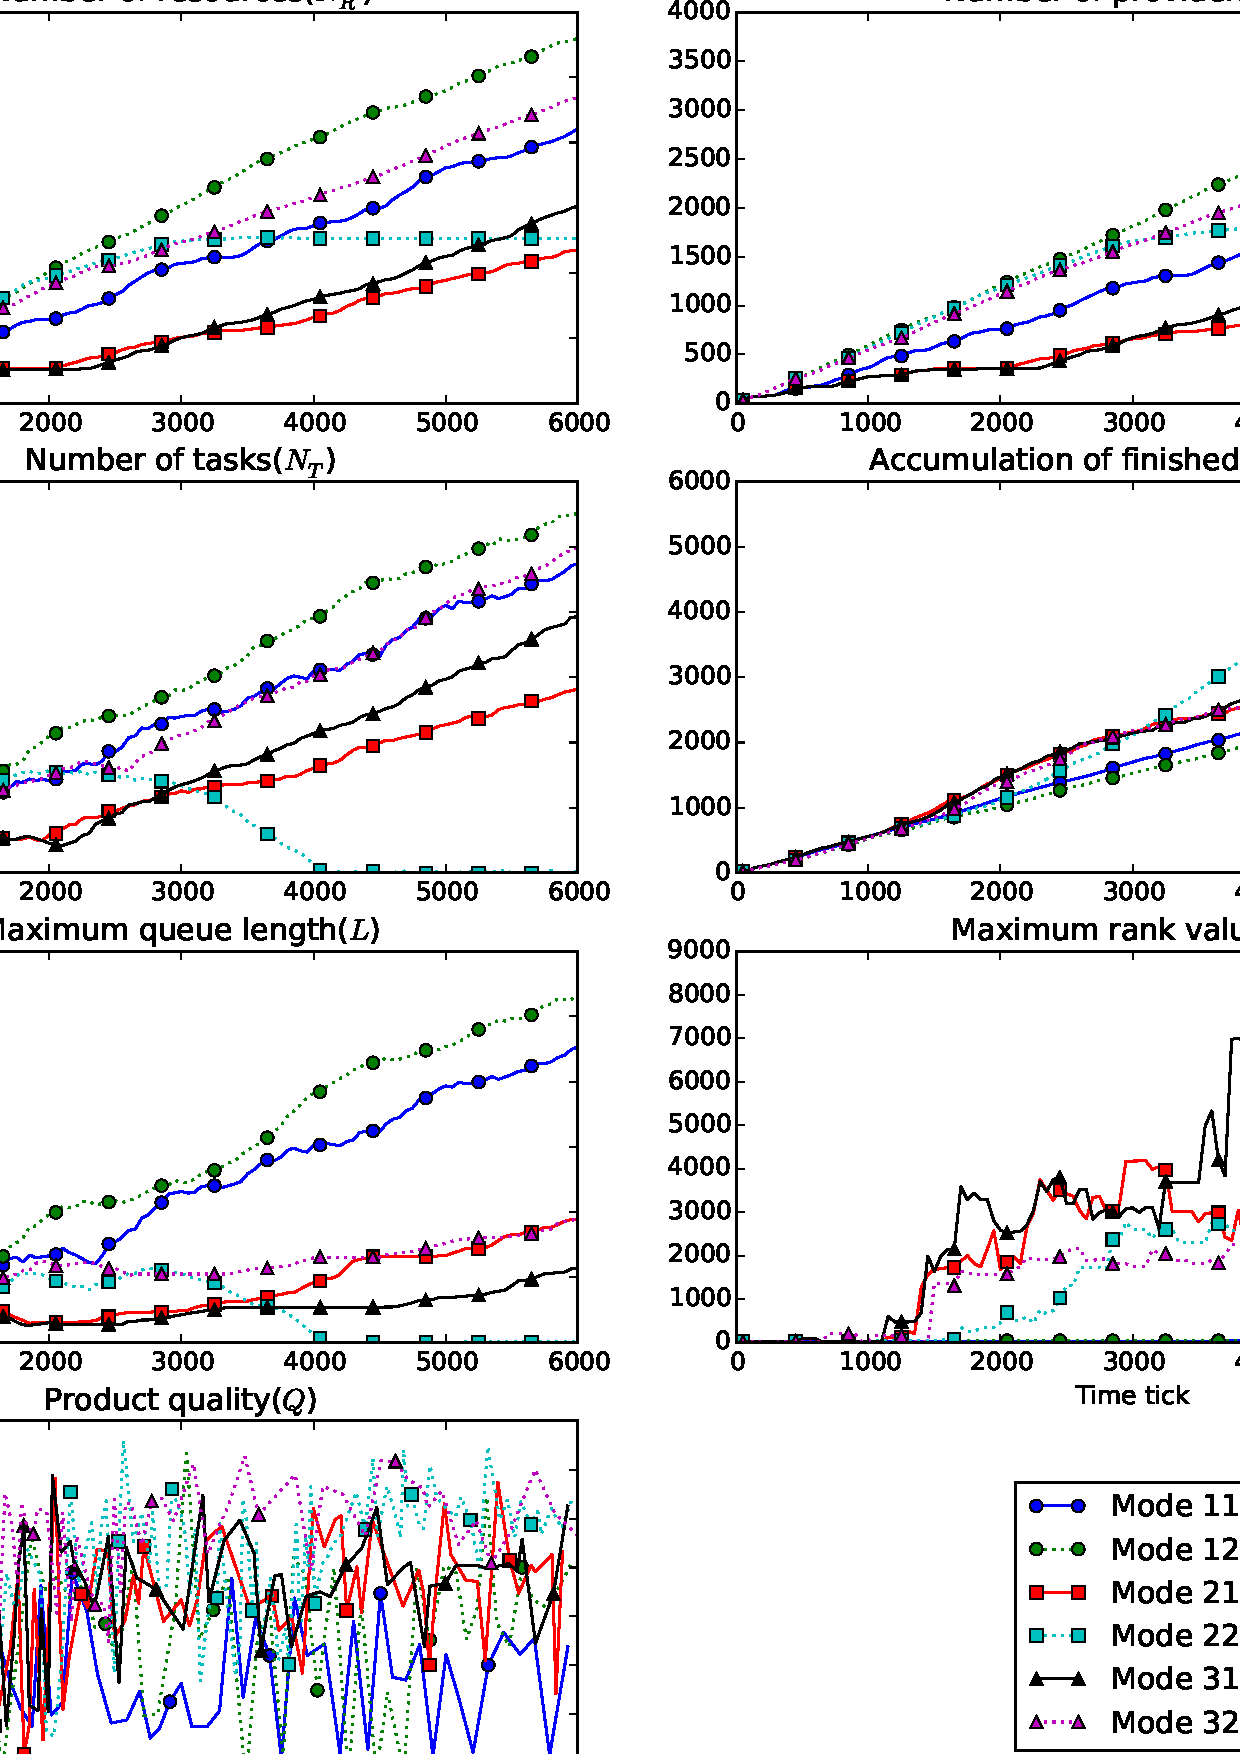
\includegraphics[width=\textwidth]{Data/out.pdf}
    \caption{Observed variable change with time}
    \label{fig:out}
\end{figure}
\begin{table}[htbp]
    \caption{Average observed values}
    \label{tab:averagevalue}
    \centering
    \scriptsize
    \begin{tabular}{lccccc}
    \toprule
    \textbf{Mode} & $\bar N_T$ & $\bar N_F$ & $\bar N_P$ & $\bar N_R $ & $\bar Q$\\
    \midrule
    Mode 11 & 1159.36 &  1644.201 &  1177.601 &  2053.727 &  8.388\\
    Mode 21 & \textit{636.769} &  \textit{2031.215} &  \textbf{692.716} &  \textbf{1066.947} &  16.016\\
    Mode 31 & 779.413 &  1996.021 &  \textit{782.272} &  \textit{1203.748} &  15.174\\
    Mode 12 & 1439.831 &  1522.923 &  1797.883 &  2954.113 &  14.057\\
    Mode 22 & \textbf{343.444} &  \textbf{2464.407} &  1316.952 &  1957.226 &  \textit{20.251}\\
    Mode 32 & 1164.409 &  1907.011 &  1597.742 &  2428.155 &  \textbf{20.652}\\

    \bottomrule
    \end{tabular}
\end{table}
we find: \begin{inparaenum}[1)]
\item Most dotted lines are above the full lines with the same series in $N_R,N_P,N_T$ means that metabolism mode need lower number of provider and resource, with the price of higher number of queue length of the tasks in resources in the system to deal with the same amount of needs, except for Mode 22. Full lines are not much above dotted lines in $N_F$ means that task processing velocity will be a little slower with the metabolism, exception also appears in Mode 22. 
\item $L$ and $N_T$ both represent the queue length of jobs, triangle and square line turned lower in $L$ meas that incubation mode can help reduce the waiting of job, these two type of line above the circle line means the incubation mode do accelerate the processing velocity.
\item Triangle lines are a little above the square lines in $N_R,N_P,N_T$ means that outsourcing mode needs more resources to operate and can only reduce the waiting of job a little.
\item There is no big difference among all the 6 modes in rank change. Provider in metabolism mode will get lower rank value for they cannot stay in the system for long, the longer stay in the system, the higher rank value provider will get. Provider in Mode 11 even will not promote their rank value, which means that the metabolism rate is very fast without incubation mode.
\item Mode 22 is a very special mode that reached the balance in 6000 ticks, that the number of provider and resource changes little with time goes by. Because our experiment setting comply \autoref{eq:balance}, the coming need capacity velocity is less than the coming capacity, Mode 12,22,32 will finally reach balance in the long run theoretically, but the appearance of service-call and metabolism itself is full of uncertainty and it's hard to predict when other metabolism related mode will get the balance.
\item With the average data value shown in \autoref{tab:averagevalue}, metabolism with incubation but not with outsourcing mode is the easiest combine mode to maintain the system, resource will self-configured and controlled to justly meet the task need.
\end{inparaenum}

% subsubsection result_and_analysis (end)
% !TEX root = Eco-Model.tex
\section{Application} % (fold)
\label{sec:application}



% section application (end)
% !TEX root = Eco-Model.tex
\section{Conclusions, Limitations, and Future Research} % (fold)
\label{sec:contributions_limitations_and_future_research}
In the extended modes we designed for cloud manufacturing ecosystem, incubation mode can realize a feasible solution for the formation of manufacturing service, shorten the job queue length and reduce the resource idle rate; outsourcing mode can cut down the amount of registered resource; metabolism mode can also cut down the amount of registered resource in price of a little higher resource idle rate. The combine of incubation and metabolism mode makes the maintenance of platform much easier.
However, we only proposed 3 extensions to combine and it may not fully describe the operation mode of cloud manufacturing system, it may also limit the evolution direction of the ecosystem, hence we will design more extensions. The assignment of service-call is oversimplified to prevent complex consequence, we will design new approaches to assign this job.
% section contributions_limitations_and_future_research (end)

\section{Acknowledgments} % (fold)
\label{sec:acknowledgments}
This work is supported by the National Natural Science Foundation of China (No. 71571161), the National High Technology Research and Development Program of China (863 Program) (No. 2015AA042101), and the Youth Funds of the Key Laboratory of Advanced Manufacturing Technology of Zhejiang Province(No. 2015QN01). 
% section acknowledgments (end)



%% 引言(准备)
%% 文献回顾(包括云制造、生态系统、制造生态系统)
%% 应用背景(包括涉及的云制造模式)
%% 模型建立
%% 模型求解及结果分析(仿真设计、实例验证)
%% 应用向导
%% 展望
%% 参考文献


%% References
%%
%% Following citation commands can be used in the body text:
%% Usage of \cite is as follows:
%%   \cite{key}         ==>>  [#]
%%   \cite[chap. 2]{key} ==>> [#, chap. 2]
%%

%% References with bibTeX database:
\bibliographystyle{../templates/Elsevier/elsarticle-num}
%\bibliographystyle{../templates/Elsevier/elsarticle-harv}
%\bibliographystyle{../templates/Elsevier/elsarticle-num-names}
%\bibliographystyle{../templates/Elsevier/model1a-num-names}
%\bibliographystyle{../templates/Elsevier/model1b-num-names}
%\bibliographystyle{../templates/Elsevier/model1c-num-names}
%\bibliographystyle{../templates/Elsevier/model1-num-names}
%\bibliographystyle{../templates/Elsevier/model2-names}
%\bibliographystyle{../templates/Elsevier/model3a-num-names}
%\bibliographystyle{../templates/Elsevier/model3-num-names}
%\bibliographystyle{../templates/Elsevier/model4-names}
%\bibliographystyle{../templates/Elsevier/model5-names}
%\bibliographystyle{../templates/Elsevier/model6-num-names}

%\nocite{*}
\bibliography{references}
\appendix
\newpage
% !TEX root = Eco-Model.tex
\section{Parameter Setting} % (fold)
\label{sec:parameter_setting}

% section parameter_setting (end)
\end{document}

%%
%% End of file `elsarticle-template-num.tex'.